\documentclass[../ala_hataile.tex]{subfiles}
\begin{document}
	\clearpage
	
\includepdf[pages=14, pagecommand={}]{sisasivut_19062018.pdf}
	\twocolumn[\section{Chemicum}]
	Kaikki kemian kurssit järjestetään Chemicumissa,
	A.~I.~Virtasen aukion laidalla
	olevassa rakennuksessa, jota on osuvasti
	kuvattu suuren WC:n näköiseksi valkoisen
	laatoituksensa takia. Chemicumin pääsisäänkäynti
	on aukion laidalla olevan lasiseinän
	kohdalla. Ilman avaimia
	sisään pääsee ko.\,oven lisäksi vain heti sen
	vieressä olevasta väliköstä.
	
	Chemicumin oven takaa paljastuu aula,
	jonka reunoilla ovat kaikki luentosalit. Ensimmäisenä
	vasemmalla on suuri luentosali
	A110, jossa luennoidaan kaikki suurimmat
	kurssit. Salin viereisellä seinällä ovat
	kurssi-ilmoitustaulut, joille ilmestyy luentoilmoituksia
	vapaavalintaisista ja syventävistä
	kursseista.
	
	Hieman edempänä oikealla, naulakkoja
	vastapäätä on lasinen koppi, jossa asustavat vahtimestarit. Opintotoimisto on vahtimestareiden kopin takana.
	
	Vahtimestareiden kopin jälkeen ennen
	vitriinejä on sisäänkäynti pieneen luentosaliin
	eli A129:ään, jossa käydään kaikki
	ne massakurssit, jotka eivät A110:n aikatauluun
	sovi. Vitriinien jälkeen molemmin
	puolin kapenevaa aulaa on neljä seminaarisalia,
	jotka tulevat sivu\-tieteen\-ala\-opiskelijalle
	tutuksi vain syventävillä kursseilla tai orgaanisen
	kemian laskuharjoituksissa (tai
	tähtitieteen luennoilla, mutta se onkin jo
	toinen tarina). Aulan vasemmalla seinustalla
	on lisää ilmoitustauluja, joille ilmestyvät
	aikanaan kokeiden tulokset.
	Aulan perällä siintää limuautomaatti, jonka lähellä on enää vain seminaari\-huoneita ja peda\-lehtorien toimisto. 4.\,kerroksen aulassa toimii kemian opinto\-paja iltapäivisin.
	
	Palataanpa taas pääovelle.
	Ennen vahtimestareiden koppia lattiasta
	kohoaa portaikko korkeuksiin. Portaikon
	varrella ja päässä ovat penkeillä ja pöydillä varustetut kerrosaulat, jotka ovat hyviä
	paikkoja vaikkapa laskuharjoitusten tekoon,
	sillä ne ovat verrattain rauhallisia.
	Kerrosauloista pääsee myös laboratorioihin. Toisesta kerroksesta
	pääsee suureen luontosaliin takaovesta,
	joka käyttö on erittäin toivottavaa, jos saapuu
	luennolle myöhässä tai haluaa sellaiselta
	poistua kesken kaiken. Laiskemmille
	ihmisille on portaiden korvikkeeksi tarjolla
	hissi, joka on piilotettu suuren luentosalin
	viereiseen nurkkaukseen. 
	
	Jos kääntyy pääovesta oikealle, pääsee pieneen lasivälikköön,
	jonka toisella puolella on
	B-siipi. Välikön takana vasemmalla
	on UniCafe, kun taas oikealta puolelta paljastuu 
	ATK- ja opiskelutilan takaa hieman
	viihtyisämpi huone, jonka käyttötarkoituksen
	arvaa helposti sisältä kuuluvasta
	älämölöstä. Kyseessä on opintososiaalinen
	tila, eli tuttavallisemmin Opsos, jossa kemian
	opiskelijoiden ainejärjestö HYK majailee.
	Opsosissa lattiatila täyttyy sohvista,
	joiden pehmusteet täyttyvät rupattelevista
	tai pelailevista opiskelijoista. Onpa joidenkin
	nähty jopa tekevän niillä laskuharjoituksiaan!
	
	Opsosin vakiovarusteisiin kuuluvat
	opiskelijoiden lisäksi Aku Ankan vuosikerrat
	usean vuoden takaa, mittava valikoima
	lauta- ja korttipelejä, kemian oppikirjoja
	ja kansioita täynnä vanhoja kokeita kaikilta
	kemian kursseilta ja monen muunkin
	aineen kursseilta. Koska kurssikokeissa
	tuppaa olemaan samoja kysymyksiä tai teemoja
	vuodesta toiseen, vanhojen kokeiden
	pläräämisestä voi olla merkittävää hyötyä
	kokeisiin valmistautuessa.
	Lisäksi Opsosista voi ostaa haalarimerkkejä, kemian alan sanastoja,
	labratakkeja, suojalaseja ja ennen kaikkea
	suolaista ja makeaa purtavaa.
	
	Jos tosin hetkeksi lopetetaan Opsosissa löhöäminen ja siirrytään asiaan, 
	niin seuraavan lasioven takana on B-siiven aula, 
	jossa on neljä opiskelijoiden käytössä olevaa tietokonetta, 
	tulostin sekä koululaisille suunnattu kemianluokka Gadolin. Käytävällä edempänä ovat
	harjoitustyölaboratoriot, joista ensimmäisessä harjoitellaan epäorgaanisen kemian
	töitä. ``Kulmalabran'' vieressä on
	radio- ja fysikaalisen kemian sekä opettajankoulutuksen
	yhteinen harjoituslaboratorio
	ja loput tämän kerroksen harjoitustyösaleista
	ovat orgaanisen ja epäorgaanisen
	kemian yhteiskäytössä. Käytävillä oleviin
	sinisiin vaatekaappeihin voi jättää tavaransa
	laboratoriopäivän ajaksi.
	\begin{figure}[b!]
		\centering
		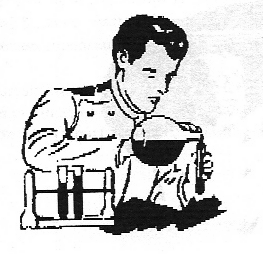
\includegraphics[width=\columnwidth]{kemistikaataa.png}
	\end{figure}
	
	Ai niin, siinä labroja vastapäätä on myös lasiovi, joka johtaa taas
	uuteen maailmaan: kemian opettajan\-koulutus\-yksikköön.
	Tässä kotoisassa paikassa
	ope\-opiskelijat (ja välillä muutkin) vaihtavat
	kuulumisia, ryystävät kahvia ja jopa
	opiskelevat.
	
	\twocolumn[\section{Kemian kursseja}]
	\subsection*{Perusopinnot}
	\subsubsection*{Kemian perusteet (5~op)}
	Kurssi on Atomit, molekyylit ja vuorovaikutukset
	"-kurssi typistetyssä muodossa
	erityisesti niille sivu\-tieteen\-ala\-opiskelijoille,
	jotka haluavat vain saada pintaraapaisun
	aineeseen.
	
	\subsubsection*{Atomit, molekyylit ja vuorovaikutukset (5~op)}
	Tämä kurssi on pakollinen, ja sillä käydään
	kemian perussanastoa ja osaamistoa. Kurssi
	alkaa uusista termeistä kuten entropia
	ja Gibbsin energia, mutta sisältää osittain
	myös lukion kertausta sekä fysiikan että
	kemian puolelta. Kurssiin kuuluu
	sähköiset (kotikoneella tehtävät) Mastering
	Chemistry "-tehtävät.
	\subsubsection*{Energia, reaktiivisuus ja kemiallinen tasapaino (5~op)}
	Tämä kurssi on suoraa jatkumoa
	AMV:stä ja myös pakollinen kaikille kemian
	opiskelijoille, Tarkoitus on laajentaa
	osaamista reaktion tapahtumisesta ja etenemisestä,
	sähkökemiasta, sekä hapoista ja
	emäksistä. Kurssilla jatkuvat myös
	Mastering Chemistry "-tehtävät. Kurssi
	vastaa joidenkin vanhempien opiskelijoiden
	ennen vuotta~2014 käymää Yleinen
	kemia~II "-kurssia.
	\subsubsection*{Orgaaninen kemia~I (5~op)}
	Orgaaninen kemia~I on pakollinen kaikille
	kemian opiskelijoille. Tällä kurssilla
	käydään lukiosta jo tuttua orgaanisten molekyylien
	nimeämistä ja erilaisia reaktioita.
	Kurssin jälkeen kuuluisi osata sanoa miten
	tietty funktionaalinen ryhmä saadaan aikaan ja
	mitä reaktioita sillä voidaan tehdä. Kurssilla
	on vapaaehtoiset tehtävät, joista saa pisteitä
	loppuarvosteluun.
	
	\subsubsection*{Kemian perustyöt (5~op)}
	Kemian perustyöt on fuksien ensimmäinen
	laboratorio\-kurssi ja sitä varten tarvitaan labra\-takki.
	Kurssi on pakollinen kaikille kemian opiskelijoille.
	Kurssilla käydään ensiksi läpi laboratorio\-työskentelyn 
	turvallisuus\-säännöt vallan tarkasti, jonka jälkeen
	päästään tekemään perus\-reaktioita
	ja "-titrauksia, samalla täyttäen vastauksia paperi\-nipun
	kysymyksiin. Lisäksi kurssi sisältää fuksin ensimmäiset 
	synteesityöt, joiden jollain tasolla tulisi olla tuttuja jo Orgaaninen kemia~I "-kurssilta.
	
	\subsubsection*{Epäorgaaninen kemia (5~op)}
Kurssilla käydään läpi kaikkea epä\-orgaaniseen
	kemiaan liittyvää mikro\-piireistä
	kide\-virheisiin. Erityisen hyvin kurssin jälkeen
	kuuluisi olla hallussa alkuaineiden
	jaksollinen järjestelmä ja siihen liittyvät
	säännöllisyydet.
	
	\subsection*{Aineopinnot}
	\subsubsection*{Liuoskemia (5~op)}
	Liuoskemian kurssilla nimen mukaisesti
	opitaan kaikenlaista liuoksista, pääpaino liuos\-tasa\-paino\-laskuissa. Kurssilla opitaan
	muun muassa tekemään paperin ja viivottimen
	kanssa kemistin arvio tietyn konsentraatioisten
	happo-emäsliuosten ja seosten pH:sta.
	
	\subsubsection*{Biologinen kemia (5~op)}
	Kurssi on pakollinen varsinaisille kemian\-opiskelijoille,
	ja sillä käydään proteiineja, entsyymejä,
	ja nukleiini\-happoja rakenteelta
	ja toiminnalta. Kurssilla on vapaaehtoiset
	tehtävät. Kurssin jälkeen tutuksi ovat tulleet
	myös aminohapot, peptidit ja lipidit.
	
	\subsubsection*{Termodynamiikka ja dynamiikka (5~op)}
Termodynamiikka
	ja dynamiikka tai tutummin
	Teddy on fuksien ensimmäinen fysikaalisen
	kemian kurssi. Kurssilla on myös pakolliset
	laskutehtävät ja niille tuutoroinnit.
	Varsinkin jos Matematiikkaa kemisteille
	tuotti ongelmia, älkää pelätkö käydä tuutoroinneissa
	ja nykimässä hihasta jokaista
	vanhempaa opiskelijaa joka ei lähde karkuun
	oppikirjan nähdessään. Kurssilla käydään
	pääasiassa kaasujen termodynamiikkaa,
	eli painetta, lämpöä ja reaktioita.
	
	\subsubsection*{Orgaaninen kemia~II (5~op)}
	Orgaaninen kemia~II sukeltaa syvemmälle
	orgaanisen kemian maailmaan, jota
	hallitsevat pienet, kaarevat nuolet, jotka
	kuvaavat elektronien vipellystä atomilta
	toiselle. Kurssilla tutustutaan tärkeimpien
	orgaanisten yhdisteryhmien tyypillisiin reaktioihin.
	Pelkältä ulkoluvulta tuntuvissa
	reaktiomekanismeissa on järkeäkin takana,
	mutta valitettavasti tämä selviää vasta
	orgaanisen kemian syventävillä kursseilla.
	Vanha kunnon ulkoluku on siis hyvä hallita.
	Kurssilla on vapaaehtoisia laskuharjoituksia,
	joista voi saada tuntuvasti bonusta
	kokeeseen.
	\subsubsection*{Yhdisteiden rakenteiden selvittäminen (5~op)}
	Orgaaniset reaktiot ovat aika hankalia, jos ei osaa tunnistaa lähtöaineita eikä lopputuotteita.
	YRS opettaa tulkitsemaan
	UV/Vis-, IR-, NMR- ja massa\-spektro\-metrialla
	saatua dataa, jolla selviää yhdisteen
	kuin yhdisteen rakenne. Kurssi pidetään
	luentosalissa, mutta tyyliltään se on enemmänkin
	harjoitustyökurssi.
	
	\begin{figure}[!b]
		\centering
		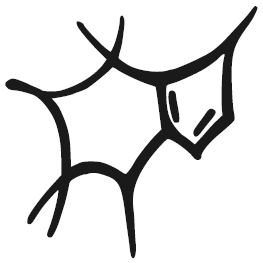
\includegraphics[width=0.8\columnwidth]{bentseeni.png}
	\end{figure}
	\subsubsection*{Orgaanisen kemian työt (5+5~op)}
	Jos jokin haisee, se on orgaaninen kemia!
	Muut opiskelijat huomaavat kyllä,
	milloin orgaanisen kemian laboratoriotyöt
	ovat käynnissä. Ykköstöissä tehdään useita
	synteesejä ja lopuksi analysoidaan perinteisin
	menetelmin assistenttien tekemä kemikaalicocktail.
	Kakkostöissä tehdään pidempiä ja vaikeampia synteesejä.
	
	\subsubsection*{Epäorgaanisen kemian työt (5+5~op)}
	Epäorgaanisen kemian työt "-kursseilla opitaan
	toteuttamaan kemistin perinteisimmät ja 
	tavallisimmat kvantitatiiviset ja kvalitatiiviset
	analyysimenetelmät. Jos harjoittelulaboratorion
	pöydiltä löytyy tahroja, ne ovat todennäköisesti
	näiltä kursseilta. Kurssin lopuksi suunnitellaan ja toteutetaan
	itse analyysireitti assistentin antamalle suolaseokselle.
	\subsubsection*{Molekyylien rakenne ja spektroskopia (5~op)}
	Atomer eller molekyler? Tuntuivatko
	AMV:n ja ERK:n molekyyliorbitaalit abstrakteilta?
	MORS kertoo, mistä ja miksi ne
	tulevat. Kurssilla perehdytään kemiallisten
	yhdisteiden rakenteeseen atomi- ja pienemmälläkin
	tasolla. Derivointi ja integrointi
	on syytä olla hallussa ennen tätä kurssia,
	muuten aaltoyhtälöt lainehtivat aivan muualla
	kuin paperilla. Kurssilla on pakolliset
	laskuharjoitukset, joista on saatava määrätty
	määrä pisteitä, jotta saa tenttioikeuden.
	Laskuharjoituksista voi saada myös lisäpisteitä
	kokeeseen.
	\subsubsection*{Fysikaalisen kemian työt (5~op)}
	Nämä harjoitustyökurssit konkretisoivat
	MORS:in ja TEDDY:n asioita. Kursseihin
	kuuluu sekä kokeellisia töitä mittausvälineillä
	että puhtaasti laskennallisia töitä
	tietokoneella. Jokaisesta työstä tehdään
	kirjallinen työselostus, joista jokaiseen on
	syytä varata pitkälti toista kymmentä tuntia
	aikaa.
	
	\subsection*{Muut opinnot}
	\subsubsection*{Matematiikkaa kemisteille (5~op)}
	Matematiikkaa kemisteille on pakollinen
	varsinaisille kemian\-opiskelijoille, ellei sitä korvaa fysiikan kurssilla Matemaattiset apuneuvot~I (FYS1010). Matematiikka alkaa tasolta, jolta lukion pitkä matematiikka auttaa matkaan, mutta ei kannata
	ylpistyä tai huomaat miettiväsi pakollisia
	tehtäviä varten yhtäkkiä miten differentiaali\-laskut kolmen muuttujan suhteen pallo\-koordinaatistossa
	taas menivätkään. Kurssi
	kannattaa käydä kunnolla seuraten läpi sillä
	tietoja edellytetään fysikaalisen kemian pakollisilla
	kursseilla. Kurssilla on pakollisia
	laskareita varten tuutorointeja, joilla vanhempi
	opiskelija on paikalla vastaamassa
	kysymyksiin ja auttamassa laskemaan jos
	ei muuten suju.
	
	\twocolumn[\section{Kemia sivutieteenalana}]
	Toisten koulutusohjelmien opiskelijoille kemia tarjoaa jonkin verran vaihtoehtoja. Ilman laboratoriotöitä
	ei opintokokonaisuuksista selviä,
	onhan laboratorio juuri se paikka, jossa
	kemiaa oikeasti tehdään! 
	
	Tässä oppaassa
	ei yritetäkään kertoa, mitkä kurssit täytyy
	/ kannattaa valita, vaan siinä asiassa on
	parasta kääntyä opinto\-neuvonnan puoleen. Tavallisesti sivu\-tieteen\-ala\-opiskelija
	suorittaa perusopinnot ja halutessaan myös
	aine\-opinnot. Opettajaopiskelijoille aine\-opinnot
	ovat välttämättömät, sillä ilman
	niitä ei kemian opetusoikeutta irtoa.
	
	Kemia ei tieteenalana ole mitenkään vaikea,
	kunhan jaksaa nähdä sen eteen hieman
	vaivaa. Ensimmäisillä kursseilla on helppo
	tuudittautua valheelliseen itsevarmuuteen,
	mutta lukioasiat käydään varsin nopeasti
	ja päästään itse asiaan. Seuraavassa on lyhyet
	kuvaukset tieteen\-ala\-kokonaisuuksien
	pakollisista kursseista (huomaa, että näissäkin
	on valinnanvaraa, ks.\,opetussuunnitelmat).

Laboratoriotöissä erityisen huomioitavaa
on se, että ensimmäisellä työkerralla on oltava
paikalla tai menettää kurssipaikkansa.
Jos jostakin syystä ei pääse tulemaan, on
ko.\,ryhmän assistentille ilmoitettava siitä
ajoissa. Muutenkin laboratoriotöissä on
läsnä\-olo\-pakko toisin kuin useimmilla luennoilla.
Laboratoriossa jokaisella on oltava
mukana oma työtakki ja omat suojalasit
(näitä saa mm.\,HYKin toimistosta alias Opsosista).
	
	Toisen tieteenalan opinnot kemiassa
	aloitetaan joko kurssilla Atomit, molekyylit
	ja vuorovaikutukset tai kurssilla
	Kemian perusteet, joista jälkimmäinen on tarkoitettu matalamman lähtötason opiskelijoille. Hyvänä jatkumona tälle
	on Energia, reaktiivisuus ja kemiallinen
	tasapaino. Nämä kaksi kurssia muodostavat
	kokonaisuuden, jossa käydään peruskäsitteet
	hyvin läpi. Orgaaniseen kemiaan
	eli hiilen vipellykseen pääsee tutustumaan
	kurssissa Orgaaninen kemia~I. 
	Kemian perustöissä pääsee labraan
	tekemään yksinkertaisia reaktioita ja
	tutustumaan laboratoriovälineistöön. Näiden
	kurssien lisäksi pitää valita muutamia
	lisäkursseja, jotka voivat olla joko perustai
	aineopinnoista.
	
	Jos haluaa jatkaa kemian opintoja pidemmälle,
	pääsee opiskelemaan epäorgaanista
	ja orgaanista kemiaa syvemmin.
	Tämän lisäksi pääsee tutustumaan kemian
	fysikaalisempaan puoleen esimerkiksi termodynamiikan
	tai spektroskopian kautta.
	
	\noindent\textbf{Jos haluaa tarkempia kurssitietoja,
		niin kannattaa tutustua HYKin fuksi\-wikiin!}
\end{document}